\documentclass[smallextended]{svjour3}
\usepackage{fix-cm}
\usepackage[T1]{fontenc}
\usepackage[utf8]{inputenc}
\usepackage{mathptmx}
\usepackage{amsmath,amssymb,graphicx,booktabs,tabularx,url}
\usepackage{placeins}
\usepackage[numbers,sort&compress]{natbib}
\usepackage[hidelinks]{hyperref}
\journalname{Computing}
\smartqed
\setlength{\emergencystretch}{2em}
\newcommand{\CollegePRDelta}{-0.90780}
\newcommand{\CollegePRLoss}{9.01}
\newcommand{\CollegePRSaving}{86.44}
\newcommand{\CollegePRfiveDelta}{-0.43094}
\newcommand{\CollegePRfiveLoss}{4.28}
\newcommand{\CollegePRfiveSaving}{82.83}
\newcommand{\CollegeDegreeDelta}{0.00000}
\newcommand{\CollegeDegreeLoss}{0.00}
\newcommand{\CollegeDegreeSaving}{86.59}
\newcommand{\GrqcPRDelta}{-0.25082}
\newcommand{\GrqcPRLoss}{5.07}
\newcommand{\GrqcPRSaving}{92.70}
\newcommand{\GrqcPRfiveDelta}{0.00000}
\newcommand{\GrqcPRfiveLoss}{0.00}
\newcommand{\GrqcPRfiveSaving}{88.14}
\newcommand{\GrqcDegreeDelta}{0.00000}
\newcommand{\GrqcDegreeLoss}{0.00}
\newcommand{\GrqcDegreeSaving}{92.77}
\newcommand{\WikiPRDelta}{-40.69334}
\newcommand{\WikiPRLoss}{73.01}
\newcommand{\WikiPRSaving}{96.42}
\newcommand{\WikiPRfiveDelta}{-13.53012}
\newcommand{\WikiPRfiveLoss}{24.28}
\newcommand{\WikiPRfiveSaving}{91.98}
\newcommand{\WikiDegreeDelta}{0.00000}
\newcommand{\WikiDegreeLoss}{0.00}
\newcommand{\WikiDegreeSaving}{96.26}

\begin{document}
\title{Evaluating Candidate-Restricted Influence Maximization: Reference Budgets, Ranking Precision, and External Topologies}
\titlerunning{Evaluating candidate-restricted influence maximization}
\author{\mbox{Jiayue Sun} \and \mbox{Binbin Yong} \and \mbox{Junjie An} \and \mbox{Tianyu Bo} \and \mbox{Shuai Li}}
\authorrunning{Jiayue Sun et al.}
\institute{Jiayue Sun \at School of Artificial Intelligence, Lanzhou University, Lanzhou 730000, China
\and Binbin Yong (corresponding author) \at School of Information Science and Engineering, Lanzhou University, Lanzhou 730000, China \\
\email{yongbb14@lzu.edu.cn}
\and Junjie An, Tianyu Bo and Shuai Li \at Lanzhou University, Lanzhou, China}
\date{}
\maketitle
\begin{abstract}
Candidate restriction accelerates greedy influence maximization, yet its measured quality can depend on choices made before seeds are evaluated. We separate two such resolutions: the number of sampled worlds defining the full-candidate reference and the numerical tolerance used to truncate a ranking. A frozen external study evaluates degree, PageRank, coverage and random pools on communication, collaboration and voting topologies with 1,438--7,115 vertices, using nested budgets, disjoint 10,000-world utility evaluation and five paired computational paths. At $W=1280$, 20-node outgoing-degree pools reproduce all 15 full-greedy trajectories, whereas default PageRank loses 5.07\%, 9.01\% and 73.01\% of incremental spread. A separately frozen post-hoc control across all three budgets shows why these conclusions need resolution labels: on ca-GrQc, default PageRank-4k changes from a 5.61\% gain at $W=80$ to a 5.07\% loss at $W=1280$, but strict PageRank remains a gain at all three budgets (-11.25\%, -2.96\%, -0.54\%). CollegeMsg is unchanged by the tighter ranking and retains its loss; wiki-Vote retains a 73.96\% strict-ranking loss. Candidate pools are stable at an even tighter tolerance. Thus budget can still change seed sets and the magnitude of paired utility differences, but the apparent ca-GrQc direction reversal is not precision-robust. The evidence supports reporting reference budget, ranking tolerance, coverage, trajectory/set agreement and independent utility separately; it does not establish a universal safe pool size, convergence or expected-optimality.
\keywords{influence maximization \and Monte Carlo simulation \and candidate restriction \and evaluation methodology \and reproducibility}
\end{abstract}

\section{Introduction}
Greedy influence maximization selects seeds by estimating how much additional diffusion each candidate could generate \cite{ref1}. Restricting the eligible candidates reduces that search. Evaluating the restriction, however, requires a computational reference, and full eligibility with a finite simulation budget is itself an estimated greedy procedure. Its selected sequence can change when the number of sampled worlds changes. Reproducing that sequence, retaining independent spread, and reducing execution cost are three different outcomes.

This distinction matters when small-network results are used to justify restrictions on larger graphs. A pool of $4k$ candidates may cover most of a small graph but less than one percent of a larger one. A ranking can also be numerically close while exchanging a few candidates at a truncation boundary. Once a greedy procedure operates on the truncated pool, those exchanges can change the seed set. On a directed graph, standard PageRank emphasizes incoming importance, whereas a seed's simulated influence follows outgoing arcs. Agreement on contact graphs therefore cannot resolve topology, coverage, numerical-ranking or reference-resolution effects.

Sampling accuracy and computational efficiency are established topics in influence maximization \cite{ref2,ref8,ref9,ref16}. We do not claim a new optimization algorithm or a general discovery that Monte Carlo references can vary. Instead, we ask which empirical claims survive when candidate eligibility, finite-reference resolution, ranking resolution, independent utility and cost are evaluated together, and when observations on small contact graphs are checked on different real topologies.

The study makes three evaluation contributions. First, it separates reference budget and numerical ranking tolerance as distinct resolution choices, then traces their effects through candidate pools, seed sequences and independently evaluated spread. Second, it tests the resulting claims across communication, collaboration and voting topologies while reporting actual coverage, direction and random-world coupling. Third, it provides an auditable evidence chain that distinguishes trajectory/set agreement, utility preservation and cost. These contributions concern evaluation evidence and reproducible diagnosis. They do not establish optimality, a learned selector, a new approximation bound or superiority over efficient influence-maximization algorithms.

Figure~\ref{fig:direction-mechanism} gives a network-specific diagnostic for the clearest adverse external result. It keeps three quantities separate: the direction a ranking emphasizes, whether a truncated candidate pool contains the seeds selected by the full finite-world reference, and the independently evaluated diffusion utility. The visual motifs summarize measured structural contrasts under the recorded wiki-Vote orientation; they do not depict an observed real cascade or establish a causal direction intervention.

\begin{figure}[htbp]
\centering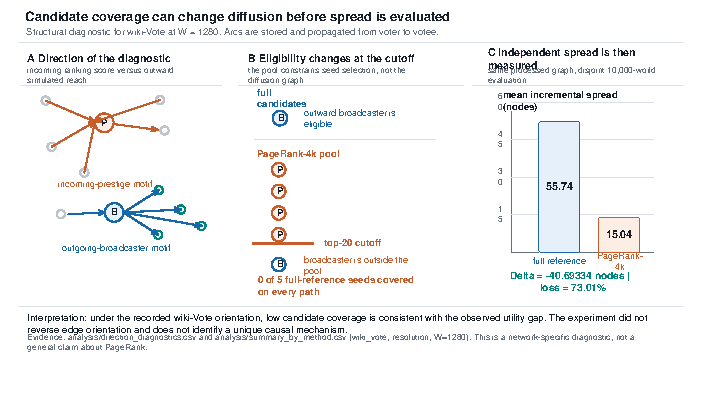
\includegraphics[width=\linewidth]{FigDirectionMechanism.pdf}
\caption{Network-specific direction--coverage diagnostic for wiki-Vote at $W=1280$. (A) Standard PageRank scores incoming-link importance, whereas the simulation propagates along stored voter-to-votee arcs; the node motifs are explanatory rather than a sampled subgraph. (B) The default PageRank-4k pool covers none of the five full-reference seeds on each of the five paths. (C) Independent 10,000-world evaluation gives mean incremental spreads of 55.73602 nodes for the full reference and 15.04268 for PageRank-4k, a paired difference of $-40.69334$ nodes (73.01\% loss). These coverage and degree facts are consistent with an incoming-ranking/outgoing-propagation mismatch under the recorded orientation. No reverse-orientation intervention was performed, so the figure does not identify a unique causal mechanism or make a general claim about PageRank.}\label{fig:direction-mechanism}
\end{figure}

\section{Related work and positioning}
The classical independent-cascade formulation relates expected reach to seed selection and provides greedy approximation results under suitable objective assumptions \cite{ref1}. CELF reduces redundant marginal evaluations using objective structure \cite{ref7}; StaticGreedy reuses fixed realizations \cite{ref8}; IMM uses a distinct sampling and guarantee framework \cite{ref2}. Our exhaustive per-round reference isolates eligibility effects without transferring those algorithms' guarantees to a different finite-world objective.

Candidate selection has been studied using local structure, including the neighbour-scale approach in \emph{Computing} \cite{ref12}, and metaheuristic search \cite{ref13}. Inductive spread estimation, such as MONSTOR+, changes the estimator using learned predictions on unseen graphs \cite{ref19}. We retain the simulator and vary seed eligibility. Consequently, the baselines here answer an attribution question, not a ranking of those published systems. Adding a trained model would require a separate training, validation and cross-graph testing design.

Benchmarking work illustrates the importance of comparable settings and implementation scope \cite{ref16}. Temporal-network influence maximization models temporal structure explicitly \cite{ref11}; aggregating an event prefix does not do so. Empirical influence estimation also requires evidence beyond observed proximity or interaction \cite{ref15}. All diffusion outcomes in this paper are simulations on observed or synthetic topologies. Messages, contacts and votes are not treated as observed information cascades. Online Resource 1 gives a source-scoped comparison of the stated focus of these works; it identifies a combination of evaluation dimensions rather than claiming that every individual dimension is new.

Our diagnostic is narrower than a comprehensive benchmark: it documents how reference reproduction, independently evaluated reach and attributed costs respond to budget and ranking resolution on specified graphs. The external validation tests the scope of the historical observations, including results that contradict an unrestricted generalization of PageRank's earlier agreement.

\section{Methods}
\subsection{Diffusion, eligibility and finite-world greedy selection}
Let $G=(V,E)$ be a directed graph. A seed set $S$ of size $k$ is active initially. Each newly activated vertex has one opportunity to activate each inactive outgoing neighbour, independently with probability $p$. Propagation stops after $h$ rounds. Let $f_h(S;\omega)$ include the seeds in total spread. The finite-world selection objective is
\begin{equation}
\widehat\sigma_W(S)=\frac{1}{W}\sum_{w=1}^{W}f_h(S;\omega_w).
\end{equation}
Given eligibility pool $C\subseteq V$, each greedy round enumerates all unselected vertices in $C$ and chooses the one maximizing the integer total $W\widehat\sigma_W$. Equal totals resolve by lexicographic original node ID. Restriction changes only seed eligibility: all arms propagate on the same complete processed graph. Full greedy means $C=V$; it is neither enumeration of all size-$k$ sets nor exact optimization of expected influence.

The main external setting is $k=5,p=.01,h=3$. Degree ranks distinct outgoing neighbours. PageRank is unweighted on the directed topology, with NetworkX 3.5 defaults: damping .85, uniform personalization and dangling-node treatment, tolerance $10^{-6}$ and at most 100 iterations \cite{networkxpr}. Iteration stops when successive vectors differ in $L_1$ norm by less than $n$ times the tolerance. Scores are sorted decreasingly, with lexical ties. This is the ranking produced by the specified stopping rule, not a certified exact PageRank ordering. Historical weighted degree is the number of outgoing observed events in the retained history; it is used only when those event counts exist.

The fixed multiplier pool contains $\min(n,4k)=20$ nodes. The coverage pool contains $\lceil .05n\rceil$ nodes. Three uniformly permuted random pools of size 20 are independently generated within each graph/path, then held fixed across budgets and coupling controls. We do not assign artificial event counts to static networks. On undirected data, observed links are converted to reciprocal arcs; this conversion is explicit.

\subsection{Random-world coupling and its scope}\label{sec:coupling}
Primary worlds hash the world identifier, propagation step, source index and target index. They share draws across arms within a condition. This step-indexed coupling gives each fixed seed set the intended independent-cascade marginal law, but its realized finite-world objective need not be monotone in the seed set. For a chain $s\to u\to v$ with horizon two, take a world in which $s\to u$ is open at step zero, $u\to v$ is closed at step zero and open at step one. Starting from $\{s\}$ reaches all three vertices; starting from $\{s,u\}$ activates $u$ too early to reach $v$ and reaches two. This counterexample does not by itself disprove submodularity.

The separately labelled fixed-edge control hashes an edge once per world. Each resulting finite objective is coverage by nodes reachable within $h$ edges and is monotone and submodular. Both controls use per-round exhaustive enumeration; no CELF or pruning is used. Fixed-edge results are not silently substituted for the historical step-coupled experiment.

World IDs derive from a frozen namespace and the graph, path, family and index. Selection IDs are nested prefixes as $W$ increases. Evaluation uses a disjoint family with $M=10,000$ worlds per path; its IDs are held across budgets. Shared IDs do not make different coupling schemes identical worlds. Separate randomization keys generate candidate pools and arm order. The complete external ID set contains 169,200 distinct identifiers, checked for collisions across graphs, paths and selection/evaluation families.

\subsection{Metrics and statistical units}
We report ordered-trajectory agreement, final-set agreement, Jaccard similarity and the first one-based divergent round. Identical sequences have first-divergence code zero. An independent paired difference on world $i$ is $d_i=f_h(S_C;\eta_i)-f_h(S_V;\eta_i)$, with
\begin{equation}
\widehat\Delta=\frac{1}{M}\sum_i d_i,\qquad
\operatorname{SE}_{\rm MC}=s(d_i)/\sqrt M.
\end{equation}
The normal interval $\widehat\Delta\pm1.96\operatorname{SE}_{\rm MC}$ is conditional on the selected sets and the simulated graph/model. It does not quantify selection-path uncertainty. Total spread includes seeds; incremental spread subtracts $k$. Incremental loss is $-100\widehat\Delta/(\widehat\sigma_{\rm full}-k)$ percent. All observed denominators are positive. Negative loss denotes a measured gain against the finite reference.

Three random-pool evaluation vectors are averaged within each path before computing a paired difference and its conditional standard error. Across-path summaries then use five path means (three in the coupling control). Reported path standard deviations include realized evaluation noise as well as selection changes; they do not isolate selection variance. Post-hoc descriptive $t$ intervals are supplied in the machine-readable tables and labelled separately. Neither worlds, paths nor conditions are independent real-network samples.

The frozen primary family compares degree-4k, PageRank-4k and the within-path random mean with full greedy at $W=1280$, separately for each graph. Two-sided exact sign tests exclude and report zero differences. Holm correction covers three comparisons within each graph. These tests address sign balance across computational paths, not the mean effect or a network population. Coverage and coupling summaries, structural diagnostics and pointwise transition intervals are descriptive. Tolerance curves use the frozen levels 0, 1, 2.5, 5, 10 and 20\% of incremental spread. No application justifies selecting one as acceptable; crossing zero or failing to reject a sign test does not establish equivalence or noninferiority.

\subsection{Implementation audit and timing}
The adapter imports the previous exhaustive Numba core byte-for-byte. Selection uses integer totals; earlier micro-unit rounding is consistent with these totals at the studied budgets. Frozen outputs preserve selected IDs, eligibility pools, every round's candidate totals, tie counts, margins and every evaluation-world spread. The independent audit reconstructs the graph from gzip text, checks source, graph and result hashes and candidate identities, regenerates full greedy score matrices and all evaluation arrays, and checks a separate scalar Python oracle for hashing and diffusion on predetermined evaluation worlds. Matching seed sets must have identical per-world values.

Two record qualifications are disclosed. The original entry point checked the frozen data-manifest file but did not enforce its raw-file hashes before running; the retrospective audit compares actual bytes with both the frozen manifest and every result's recorded hashes. The new reproduction wrapper enforces those hashes first. Also, archived graph preparation includes all rankings and diagnostic metadata. Adding recorded ranking time again would double count it. Neither frozen code nor raw results were edited to address these reporting issues.

Selection timings exclude world preparation, graph setup and evaluation. For a warm-process deployment estimate, we add a separate post-hoc five-repeat measurement of parsing, compressed-sparse-row construction and one method's ranking/pool construction to the frozen selection-world preparation and selection time. A verification-inclusive estimate further adds independent-world preparation and evaluation. These assembled costs are hybrid estimates, not directly timed end-to-end runs. Imports, just-in-time compilation, downloading and output writing are excluded. Five additional randomized frozen repeats at path 1101, $W=320$ check timing variability and deterministic outcomes. Reported peak memory is the psutil process-lifetime peak, not a reset per-condition allocation.

\subsection{AI assistance and human review}
OpenAI Codex assisted code development, verification scripts, analysis, figure generation and manuscript drafting in this revision. Outputs are linked to frozen records and executable scripts. This assistance does not constitute human scientific approval. The authors must confirm the complete disclosure, check interpretations and take responsibility for the final manuscript before submission.

\section{Evidence layers and data}
\subsection{Historical studies}
The first archived study has 42 conditions and 168 arm executions, using two paths, $W=20,80,320$ and $M=2000$. Its later diagnostics are historical exploratory evidence. A separate locally frozen extension has 520 conditions and 4,680 arm executions, ten paths on four contact-derived graphs, budgets up to 5120 and $M=10,000$. It includes alternative rankings, propagation parameters, seed budgets, coupling controls and two 2,000-node synthetic graphs. Neither layer is public preregistration.

Contact data originate from the InVS workplace, SFHH conference and rural Kenya studies \cite{ref3,ref4,ref5,ref6}. Retaining the first 65\% of complete timestamp groups yields 91, 212, 402 and 75 nodes, respectively. The synthetic controls use preferential attachment and a four-block stochastic block model \cite{ref17,ref18}. Their topology-derived weights are not independent historical-event evidence. These layers remain immutable and their complete results accompany the local reproduction materials.

\subsection{External topologies and preprocessing}
The external set was chosen before inspecting its seeds or utilities, using source provenance, structural diversity and larger graph size. Public SNAP files provide the three topologies \cite{snap}. Outcome-blind resource preflight persisted timing/resource records rather than selected sets or utility. It used $W=80,320$ and $M=1000$. That preflight is not part of the main utility evidence.

\begin{table}[htbp]
\caption{Frozen external topologies. Arcs are directed propagation arcs after preprocessing. The coverage pools use $\lceil .05n\rceil$. The raw ca-GrQc page counts 5,242 nodes; see the endpoint rule in the text.}\label{tab:data}
\begin{tabular}{lrrrr}
\toprule
Graph & Nodes & Arcs & 4k fraction & 5\% pool \\
\midrule
CollegeMsg & 1,438 & 13,397 & 1.391\% & 72 \\
ca-GrQc & 5,241 & 28,968 & 0.382\% & 263 \\
wiki-Vote & 7,115 & 103,689 & 0.281\% & 356 \\
\bottomrule
\end{tabular}
\end{table}

CollegeMsg records sender, receiver and timestamp \cite{college}. We retain the first $\lfloor .65T\rfloor$ unique timestamp groups, where $T=58,911$, including all rows through Unix timestamp 1085640224. This yields 38,939 non-self message events and the topology in Table~\ref{tab:data}. Historical weighting counts messages emitted by each source. Diffusion uses uniform $p$ on distinct retained directed pairs, not a message-frequency transmission model. The unused later events are not held-out influence cascades.

ca-GrQc is an undirected coauthorship network \cite{grqc}. Self-loops are removed, pairs deduplicated and reciprocal arcs constructed. Frozen code collects vertices from non-self edges, giving 5,241 vertices. Raw node 12295 appears only in a self-loop and is consequently absent. The pre-outcome manifest already recorded this size/hash, although the prose phrase ``nodes appearing in edges'' was ambiguous about filtering order. We explicitly report the implemented endpoint rule rather than asserting retention of the entire raw node universe. Reinserting an isolate changes lexical indices and hash draws, so no identical-path claim is made for a 5,242-node representation.

wiki-Vote has arcs from voters to users voted upon \cite{signed,links}. Outgoing propagation is a simulation convention, not evidence that votes transmit adoption in that direction. This direction differs from incoming PageRank importance. Neither static file supplies event counts or observed cascades, and neither receives a historical-weighted ranking. The three processed graphs have, respectively, 2, 354 and 24 weak components; all retained components are included, with no outcome-based subgraph selection.

\subsection{Frozen external matrix}
The primary resolution matrix contains $3\times5\times3=45$ conditions: three graphs, paths 1101--1105, and $W=80,320,1280$ under step coupling. Nine further conditions use fixed-edge coupling at $W=320$ on paths 1101--1103. Every condition evaluates full, degree-4k, PageRank-4k, degree-5\%, PageRank-5\% and three random-4k pools. CollegeMsg additionally evaluates historical-weighted 4k and 5\% pools. This yields 54 conditions and 468 executed arms, all retained. Each uses 10,000 independent evaluation worlds.

The external study does not reach $W=5120$. Its purpose is a bounded comparison over the frozen budgets, not convergence assessment. Higher-budget convergence claims have therefore been removed instead of adding an outcome-conditioned extension. The post-hoc audit and setup timings do not create new confirmatory paths. Data selection, original source hashes, processed graph hashes, code snapshot, full configuration and result indices are retained separately from this submission-preparation package.

The audit detected changed PageRank candidates when tightening numerical tolerance. A separate post-hoc protocol was then frozen before inspecting the resulting diffusion outcomes. It first reran both PageRank pool sizes at tolerance $10^{-12}$, with at most 1,000 iterations, on all three graphs and five original $W=1280$ paths. A second protocol, also frozen before its new outputs, added the same restricted arms at $W=80,320$ on the same paths. Thus the two post-hoc layers contain 45 conditions and 90 restricted-arm executions; they reuse the original graphs, world prefixes, full references and disjoint evaluation worlds. Pool membership agrees at $10^{-14}$. These diagnostics do not add independent paths, alter graph inclusion or modify the prespecified testing family. Original results are preserved.

\section{Results}
\subsection{External validation limits transfer of ranking results}
Table~\ref{tab:primary} reports the frozen primary external results. At $W=1280$, degree-4k exactly reproduces all five ordered references on each graph, using only 20 eligible vertices. Default-tolerance PageRank-4k matches none of those trajectories and has mean paired differences of \GrqcPRDelta{}, \CollegePRDelta{} and \WikiPRDelta{} on ca-GrQc, CollegeMsg and wiki-Vote. Corresponding incremental losses are \GrqcPRLoss{}, \CollegePRLoss{} and \WikiPRLoss{} percent. Every default-tolerance PageRank-4k path difference is negative. The numerical-precision qualification below is necessary for interpreting these values.
\begin{table}[htbp]
\caption{Frozen external results at $W=1280$, five paths per graph. PageRank uses a 20-node pool and default solver tolerance. Loss is normalized by full-reference spread beyond the five seeds. Degree agreement is ordered-trajectory agreement.}\label{tab:primary}
\begin{tabular}{lrrrr}
\toprule
Graph & Full extra & PR difference & PR loss (\%) & Degree \\
\midrule
ca-GrQc & 4.934 & -0.25082 & 5.07 & 5/5 \\
CollegeMsg & 10.072 & -0.90780 & 9.01 & 5/5 \\
wiki-Vote & 55.736 & -40.69334 & 73.01 & 5/5 \\
\bottomrule
\end{tabular}
\end{table}


These findings contrast with the historical contact-graph extension, where PageRank-4k reproduced 40/40 ordered references at $W=5120$ and degree-4k reproduced 39/40. The external results retain degree agreement at the tested highest budget but prevent generalizing the earlier PageRank result across topology, direction and coverage. They do not show that every restricted method loses utility, or that degree is expected-optimal.

The primary sign-test result is equally explicit. Each PageRank and random-mean comparison has five negative path differences, unadjusted $p=.0625$ and within-graph Holm $p=.1875$. Degree comparisons have five exact zeros and assigned $p=1$. With five paths, the prespecified two-sided sign test cannot attain .05 even when every nonzero sign agrees. Thus no primary comparison is declared significant after correction. This test-resolution limit is reported alongside measured effects, not interpreted as equivalence or absence of a loss.

\begin{figure}[htbp]
\centering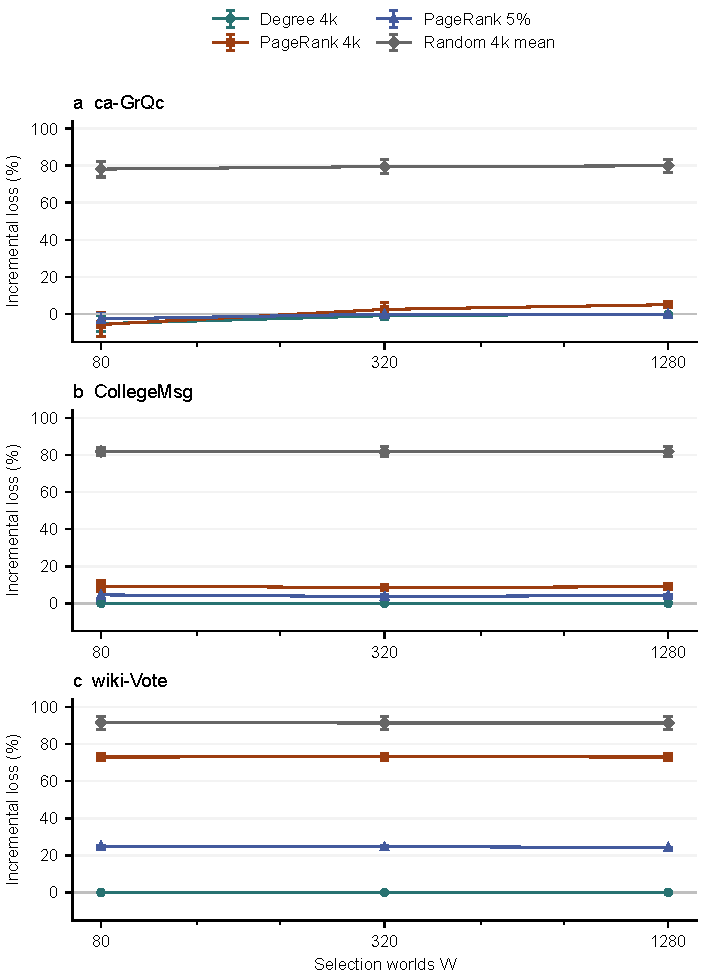
\includegraphics[width=\linewidth]{Fig1.pdf}
\caption{Frozen main-matrix incremental loss relative to each budget's full reference; PageRank uses default tolerance. Points are means of five computational paths; bars are path standard deviations. Random-pool repeats are averaged within each path first. Negative loss denotes independently measured gain against the finite reference. Graph panels retain a common percentage scale. Complete method summaries and source data accompany Online Resource 1}\label{fig:loss}
\end{figure}

\subsection{Ranking precision changes one apparent budget reversal}
The strict-tolerance budget control answers a question left open by the original $W=1280$ diagnostic. Table~\ref{tab:precision-budget} and Fig.~\ref{fig:precision-budget} show losses at all three budgets. On ca-GrQc, default PageRank-4k goes from a 5.61\% gain at $W=80$ to losses of 2.53\% and 5.07\%. Strict PageRank-4k uses a pool differing in two of 20 candidates, is stable at $10^{-14}$, and instead has gains of 11.25\%, 2.96\% and 0.54\%. Its selected sets nevertheless change on 3/5 paths from $W=80$ to 320 and 2/5 from 320 to 1280; its mean paired difference decreases by 0.34766 and 0.11196 nodes, respectively. Thus reference budget still changes the realized candidate-restriction evaluation, but the default solver's gain-to-loss direction reversal is not a precision-robust result.

CollegeMsg's strict and default pools, seeds and evaluations are identical at every budget, retaining 4k losses of 9.33\%, 8.52\% and 9.01\%. On wiki-Vote, a one-node 4k-pool exchange is stable at $10^{-14}$ and strict losses remain 74.05\%, 74.05\% and 73.96\%; its 5\% losses remain near 25\%. These contrasts distinguish a solver-sensitive collaboration result from two stable negative external results. They do not license a new significance test or a claim that any sign change alone is practically consequential.
\begin{table}[htbp]
\caption{Post-hoc PageRank loss across budgets. Each entry is the mean incremental-loss percentage across five original paths at $W=80/320/1280$. Default uses NetworkX tolerance $10^{-6}$; strict uses $10^{-12}$, whose pool is unchanged at $10^{-14}$. Pool Jaccard compares default and strict candidates. This is a numerical sensitivity analysis, not a new primary test family.}\label{tab:precision-budget}
\begin{tabular}{llrrr}
\toprule
Graph & Pool & Default loss (\%) & Strict loss (\%) & Pool Jaccard \\
\midrule
ca-GrQc & 4k & -5.61 / 2.53 / 5.07 & -11.25 / -2.96 / -0.54 & 0.818 \\
ca-GrQc & 5\% & -2.62 / 0.00 / 0.00 & -2.62 / 0.00 / 0.00 & 0.977 \\
CollegeMsg & 4k & 9.33 / 8.52 / 9.01 & 9.33 / 8.52 / 9.01 & 1.000 \\
CollegeMsg & 5\% & 4.57 / 3.72 / 4.28 & 4.57 / 3.72 / 4.28 & 1.000 \\
wiki-Vote & 4k & 73.01 / 73.06 / 73.01 & 74.05 / 74.05 / 73.96 & 0.905 \\
wiki-Vote & 5\% & 24.91 / 24.67 / 24.28 & 24.83 / 24.67 / 24.47 & 0.994 \\
\bottomrule
\end{tabular}
\end{table}

\begin{figure}[htbp]
\centering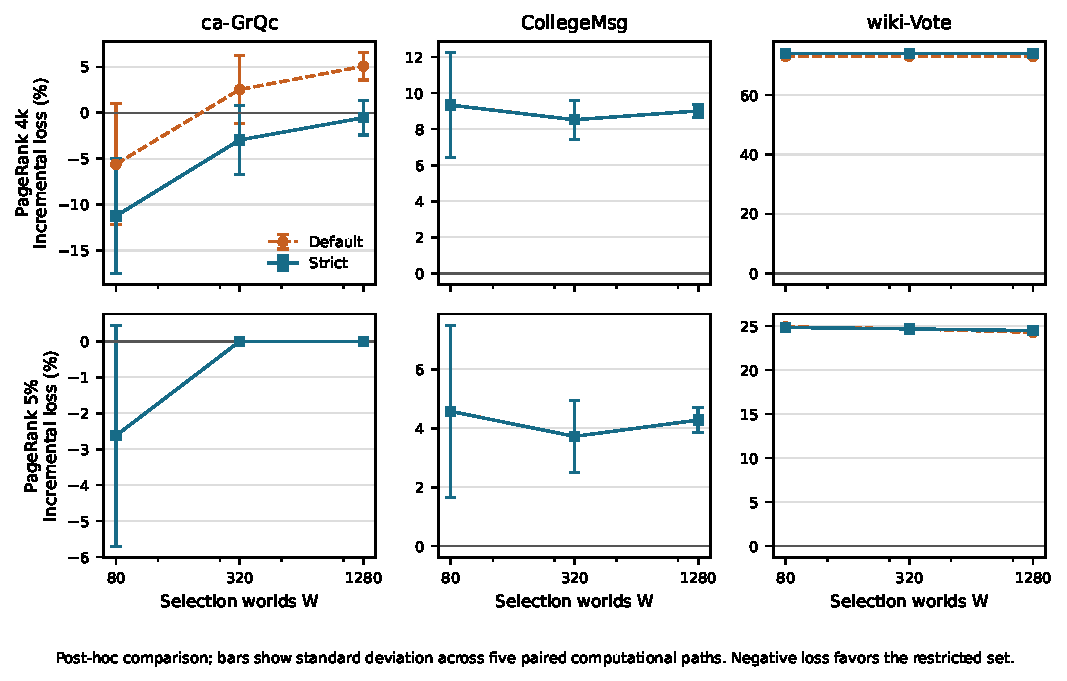
\includegraphics[width=\linewidth]{Fig4.pdf}
\caption{Post-hoc PageRank budget--precision sensitivity. Each point is the mean incremental loss over the original five paths; bars are path standard deviations. Default and strict refer to tolerances $10^{-6}$ and $10^{-12}$; strict pools agree at $10^{-14}$. Negative loss favors the restricted set. The panels show why the ca-GrQc default direction reversal cannot be generalized to the strict ranking, while CollegeMsg and wiki-Vote retain their named patterns. This is a diagnostic comparison, not a new primary test family.}\label{fig:precision-budget}
\end{figure}

\subsection{Coverage and orientation qualify the PageRank interpretation}
At the frozen default tolerance, increasing PageRank eligibility to 5\% restores ca-GrQc's five ordered references at $W=1280$. CollegeMsg's mean loss falls from \CollegePRLoss{} to \CollegePRfiveLoss{} percent, while wiki-Vote's falls from \WikiPRLoss{} to \WikiPRfiveLoss{} percent (Fig.~\ref{fig:loss}). Greater coverage helps within this implementation but does not establish a universal fraction. Historical-weighted CollegeMsg pools have mean difference $-0.25224$ at 4k, whereas the 5\% pool reproduces the full references. Fixed 4k and fixed coverage therefore answer different questions.

At $W=1280$, tightening PageRank tolerance replaces two of the 20 ca-GrQc candidates and changes all five selected sets; its mean difference becomes $+0.02608$ rather than $-0.25082$. Individual tightened differences range from $-0.0408$ to $+0.1789$, and none of its ordered traces matches full greedy. The positive mean does not establish superiority or equivalence. Thus the original small loss cannot be presented as a precision-robust property of PageRank or explained only by pool size. Complete auxiliary outputs and comparisons appear in Online Resource 1.

Post-hoc structural diagnostics give a concrete direction-related explanation for wiki-Vote (Fig.~\ref{fig:direction-mechanism}). Its default-tolerance PageRank top 20 have mean in-degree 249.75 and out-degree 56.2; its degree top 20 have mean in-degree 70.3 and out-degree 489.25. The former contain none of the five full-reference seeds on any $W=1280$ path. Even the default PageRank 5\% pool contains only one of those five seeds. These are candidate-coverage facts under the observed orientation. They are consistent with a mismatch between incoming importance and outgoing propagation, but a reverse-orientation intervention was not performed and causality is not isolated. The reciprocal ca-GrQc precision result further demonstrates that ranking accuracy must be separated from directional interpretation.

\subsection{Reference-set changes are not interchangeable with utility changes}
Table~\ref{tab:transitions} and Fig.~\ref{fig:transitions} separate changes in the full reference from changes in independently evaluated spread. Between 320 and 1280, all five ca-GrQc sets change; mean gain is 0.12720 nodes, with individual changes from $-0.0266$ to $+0.2411$. CollegeMsg changes one set, with mean gain 0.05336 across all five paths. wiki-Vote changes no final sets and has exactly zero paired gain. It does change some ordered sequences: final-set agreement and trajectory agreement must remain distinct.
\begin{table}[htbp]
\caption{Full-reference transitions under step coupling. Gain is the paired independent change in total spread; seed counts are constant. The range is across paths, not a confidence interval.}\label{tab:transitions}
\begin{tabular}{llrrr}
\toprule
Graph & Budgets & Set changed & Mean gain & Path range \\
\midrule
ca-GrQc & 80--320 & 5/5 & +0.39616 & +0.1819, +0.6139 \\
ca-GrQc & 320--1280 & 5/5 & +0.12720 & -0.0266, +0.2411 \\
CollegeMsg & 80--320 & 2/5 & +0.09994 & +0.0000, +0.2855 \\
CollegeMsg & 320--1280 & 1/5 & +0.05336 & +0.0000, +0.2668 \\
wiki-Vote & 80--320 & 0/5 & +0.00000 & +0.0000, +0.0000 \\
wiki-Vote & 320--1280 & 0/5 & +0.00000 & +0.0000, +0.0000 \\
\bottomrule
\end{tabular}
\end{table}


Of the six changed final sets in this adjacent-budget comparison, four have positive pointwise 95\% conditional Monte Carlo intervals. Two ca-GrQc intervals include zero. These unadjusted diagnostics do not determine application-specific importance. The nine unchanged sets have identical evaluation vectors, which gives exact zero paired differences rather than noisy estimates of differences between two separate runs.

At lower resolution, ca-GrQc's default-tolerance PageRank-4k mean difference changes from positive at $W=80$ to negative at $W=1280$. The new strict control shows that its corresponding strict result changes in magnitude but remains positive. Low-budget references can therefore alter evaluated seeds and utility on this topology, whereas the stronger statement that they reverse the quality direction depends on the specified ranking tolerance. This pattern is not universal: wiki-Vote's set-level reference and large loss persist across the studied budgets. The historical extension's separate 1280-to-5120 comparison changed 16/40 sets while gaining only 0.01111 nodes on average. That historical result cannot certify external stability at 1280.

\begin{figure}[htbp]
\centering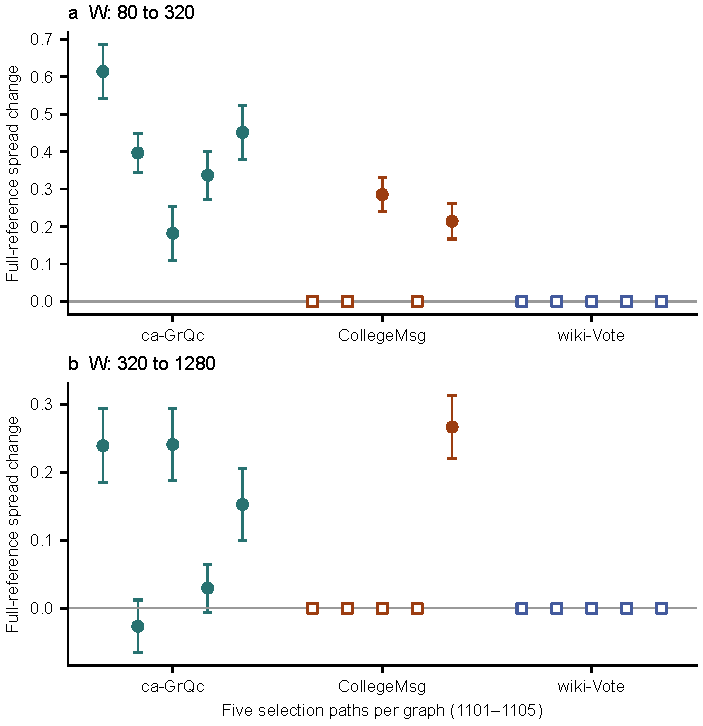
\includegraphics[width=\linewidth]{Fig2.pdf}
\caption{Full-reference paired spread changes for adjacent budgets. Each graph contributes paths 1101--1105 from left to right. Filled circles mark changed final sets; hollow squares mark unchanged sets. Bars are unadjusted 95\% normal conditional Monte Carlo intervals from 10,000 paired worlds. Panels use different vertical ranges to display the measured changes; these are not across-network confidence intervals}\label{fig:transitions}
\end{figure}

\subsection{Coupling and computational cost}
The preselected fixed-edge control does not remove the main PageRank loss pattern. At $W=320$, its mean differences are $-0.16240$ for ca-GrQc, $-0.93417$ for CollegeMsg and $-40.57597$ for wiki-Vote. Degree-4k reproduces the fixed-edge reference on all three CollegeMsg and wiki-Vote paths, but only one of three ca-GrQc paths. The three-path control is too narrow to conclude that coupling never matters. It supports reporting the coupling choice explicitly, as motivated by Section~\ref{sec:coupling}. Online Resource 1 contains the complete control results.

Table~\ref{tab:cost} distinguishes raw selection savings from hybrid verification-inclusive estimates. At $W=1280$, degree-4k reduces measured selection time by 98.40--99.67\% relative to exhaustive full eligibility. Charging relevant setup, both world families and independent evaluation reduces the estimated saving to \CollegeDegreeSaving{}--\WikiDegreeSaving{}\% across the graphs. These are comparisons with this implementation's exhaustive reference, not with optimized influence-maximization systems or a production service.
\begin{table}[htbp]
\caption{Degree-4k cost at $W=1280$. Seconds are frozen selection measurements averaged over five paths. Verification savings use the separately measured setup plus frozen world, selection and evaluation times; they are hybrid estimates, not direct end-to-end trials.}\label{tab:cost}
\begin{tabular}{lrrrr}
\toprule
Graph & Full (s) & Degree (s) & Selection (\%) & Verify (\%) \\
\midrule
ca-GrQc & 23.53 & 0.109 & 99.54 & 92.77 \\
CollegeMsg & 5.89 & 0.094 & 98.40 & 86.59 \\
wiki-Vote & 158.94 & 0.520 & 99.67 & 96.26 \\
\bottomrule
\end{tabular}
\end{table}


Figure~\ref{fig:cost} combines descriptive tolerance eligibility with the verification-inclusive cost scenario. Degree-4k passes even the zero point-estimate loss threshold on every highest-budget path. PageRank-4k passes all paths at 10\% on ca-GrQc and CollegeMsg, but none at 20\% on wiki-Vote. At 5\% coverage, PageRank passes zero loss on ca-GrQc and 5\% loss on CollegeMsg; it still passes no wiki-Vote path at 20\%. None of the random-pool path means passes 20\%. These observations show why a large cost reduction alone cannot justify a restriction. They do not guarantee future loss tolerances.

The frozen main-condition elapsed times sum to 30.65 minutes, including repeated timings. The maximum saved psutil process peak is 3.449 GiB, substantially above the smaller-world preflight. Negative values once displayed by a separate PowerShell diagnostic are not treated as experiment memory or given an unverified overflow explanation. Raw timing repetitions, setup measurements, memory records and exclusions are available in the supplementary tables and local archive.

\begin{figure}[htbp]
\centering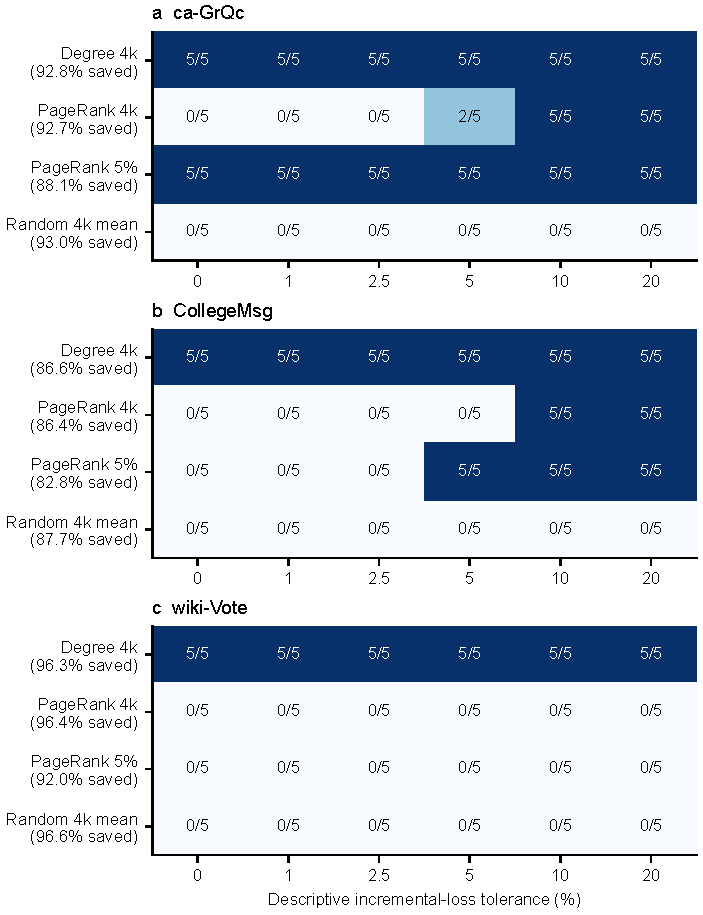
\includegraphics[width=\linewidth]{Fig3.pdf}
\caption{Descriptive loss--cost decisions for the frozen default-tolerance matrix at $W=1280$. Cells count paths whose point-estimate incremental loss is at or below the column tolerance. Row labels report mean hybrid verification-inclusive saving across all five paths, whether or not they pass. Random rows first average three pools within each path and use the mean cost of one random-pool deployment. The tolerances are illustrative, not justified application thresholds or noninferiority tests}\label{fig:cost}
\end{figure}
\FloatBarrier

\section{Discussion and limitations}
The main contribution is an evaluation distinction: finite-reference budget and numerical ranking tolerance are separate resolution choices. The ca-GrQc control demonstrates why this distinction changes interpretation. Budget still changes strict-ranking seed sets and the magnitude of the paired difference, but its default gain-to-loss reversal disappears after a stable strict pool is used. CollegeMsg's unchanged ranking preserves its loss, while wiki-Vote preserves a large loss under both resolutions. These outcomes make a more specific recommendation than merely increasing simulation worlds: report the named budget, ranking tolerance, candidate coverage, sequence/set agreement and independently evaluated utility together.

External topology changes the conclusion as well. Degree retains exact highest-budget reference agreement in this setting; PageRank's earlier contact-graph agreement does not transfer uniformly to the new networks. The persistent wiki-Vote loss is consistent with incoming-ranking versus outgoing-propagation mismatch and low full-seed coverage, but the study does not causally isolate direction. The precision-sensitive collaboration result shows why direction, coverage and numerical ranking must not be collapsed into one explanation.

Several tempting stronger conclusions remain unsupported. Reference agreement is not expected-objective optimality. Increasing the budget need not improve every realized independently evaluated set. The PageRank comparison is against a specified incoming ranking on fixed directed arcs, not all PageRank-based influence methods. A small conditional Monte Carlo interval cannot replace selection-path replication. A nonsignificant five-path sign test cannot prove negligible loss, and an illustrative tolerance cannot supply a real application's utility criterion.

The external topology range is substantially larger than the original 75--402-node contact graphs, but remains three selected networks from one repository. Different observed relations provide structural diversity, not a probability sample of social systems. The main external matrix fixes $k=5,p=.01,h=3$ and reaches only 1280 selection worlds. Larger $k$, other propagation laws, calibrated edge probabilities, direction interventions and further independent graphs may change the conclusions. Neither 1280 nor the historical 5120 budget certifies convergence to expected-spread greedy selection.

The code audit reduces the risk of arithmetic, tie-policy, provenance and coupling-implementation mistakes. It cannot validate an unmeasured real influence process. The separate scalar oracle samples predetermined worlds while complete score and evaluation replay uses the frozen core; these checks have different independence levels. The ca-GrQc endpoint rule excludes a self-loop-only vertex and is explicitly limited to the resulting graph. Timing estimates combine measurements from different runs and exclude cold-start overhead. These are material boundaries, not reasons to discard adverse results.

For future evaluations, we recommend retaining the actual eligibility fraction, ranking tolerance, named budget and coupling, per-path reference transitions, independent total and incremental spread, and a declared cost scenario. If a practical preservation claim is required, its loss threshold and uncertainty design should be justified before testing. The present records support that next design without assigning an unsupported universal threshold.

\section{Conclusion}
Candidate restriction can reproduce a particular full-greedy computation at much lower measured selection cost, but its apparent utility depends on how both the reference and the truncated ranking are resolved. Across three external topologies, strict ranking removes the ca-GrQc default budget-direction reversal without removing its budget-dependent seed changes, while CollegeMsg and wiki-Vote retain their respective losses. Paired evaluation separates changed sequences, changed sets and changed reach; explicit coverage, coupling and timing scopes prevent those outcomes from being conflated. This is an auditable characterization of the tested settings, not a new influence-maximization algorithm, a convergence result or a guarantee of general loss preservation.

\paragraph{Supplementary information.} Online Resource 1 provides the source-scoped related-work comparison, audit qualifications, the complete external aggregate matrix, post-hoc precision-budget control, primary sign tests, coupling control, timing definitions and a reproduction-file map. Machine-readable tables retain all path/arm observations and figure source data.
\section*{Statements and Declarations}
\paragraph{Funding.} This work was supported by a provincial undergraduate innovation and entrepreneurship training project.
\paragraph{Competing interests.} The authors declare that they have no competing interests.
\paragraph{Author contributions.} Jiayue Sun: conceptualization, methodology, software, validation, formal analysis, investigation, data curation, visualization, and writing---original draft. Binbin Yong: supervision, methodology, project administration, and writing---review and editing. Junjie An: software, data curation, and writing---review and editing. Tianyu Bo: validation, visualization, and writing---review and editing. Shuai Li: formal analysis, validation, and writing---review and editing. All authors read and approved the final manuscript and agreed to its submission to \textit{Computing}.
\paragraph{Data availability.} The third-party source datasets are available from the cited providers under their stated access terms. This study does not redistribute the provider archives. Source pages, retrieval records, expected SHA-256 hashes and preprocessing instructions are included in the reproducibility package accompanying the submission.
\paragraph{Code availability.} Frozen source snapshots, configurations, validators, analysis and figure-generation scripts, condition-level outputs, and figure-source tables are included in the reproducibility package supplied with the submission for editorial and peer-review access.
\paragraph{Use of AI-assisted technologies.} OpenAI Codex was used to assist code development, verification scripts, statistical analysis, figure generation, and manuscript drafting. The authors reviewed and verified the resulting work and take full responsibility for the manuscript's content.
\begin{thebibliography}{99}
\bibitem{ref1} Kempe D, Kleinberg J, Tardos É (2003) Maximizing the spread of influence through a social network. In: ACM SIGKDD, pp 137--146. \url{https://doi.org/10.1145/956750.956769}

\bibitem{ref2} Tang Y, Shi Y, Xiao X (2015) Influence maximization in near-linear time: a martingale approach. In: ACM SIGMOD, pp 1539--1554. \url{https://doi.org/10.1145/2723372.2723734}

\bibitem{ref8} Cheng S, Shen H, Huang J, Zhang G, Cheng X (2013) StaticGreedy: solving the scalability-accuracy dilemma in influence maximization. In: CIKM, pp 509--518. \url{https://doi.org/10.1145/2505515.2505541}

\bibitem{ref9} Li Y, Fan J, Wang Y, Tan K-L (2018) Influence maximization on social graphs: a survey. IEEE Transactions on Knowledge and Data Engineering 30:1852--1872. \url{https://doi.org/10.1109/TKDE.2018.2807843}

\bibitem{ref16} Arora A, Galhotra S, Ranu S (2017) Debunking the myths of influence maximization: an in-depth benchmarking study. In: SIGMOD, pp 651--666. \url{https://doi.org/10.1145/3035918.3035924}

\bibitem{ref7} Leskovec J, Krause A, Guestrin C, Faloutsos C, VanBriesen J, Glance N (2007) Cost-effective outbreak detection in networks. In: KDD, pp 420--429. \url{https://doi.org/10.1145/1281192.1281239}

\bibitem{ref12} Rui X, Yang X, Fan J, Wang Z (2020) A neighbour scale fixed approach for influence maximization in social networks. Computing 102:427--449. \url{https://doi.org/10.1007/s00607-019-00778-5}

\bibitem{ref13} Fan C, Wang Z, Zhang J, Zhao J, Rui X (2024) Influence maximization in social networks based on discrete harris hawks optimization algorithm. Computing 106:327--351. \url{https://doi.org/10.1007/s00607-023-01207-4}

\bibitem{ref19} Ko J, Kim S, Lee K, et al. (2025) Inductive influence estimation and maximization over unseen social networks under two diffusion models. Data Mining and Knowledge Discovery 39:55. \url{https://doi.org/10.1007/s10618-025-01137-z}

\bibitem{ref11} Yanchenko E, Murata T, Holme P (2024) Influence maximization on temporal networks: a review. Applied Network Science 9:16. \url{https://doi.org/10.1007/s41109-024-00625-3}

\bibitem{ref15} Aral S, Dhillon PS (2018) Social influence maximization under empirical influence models. Nature Human Behaviour 2:375--382. \url{https://doi.org/10.1038/s41562-018-0346-z}

\bibitem{networkxpr} NetworkX developers (2025) PageRank, NetworkX 3.5 documentation. \url{https://networkx.org/documentation/networkx-3.5/reference/algorithms/generated/networkx.algorithms.link_analysis.pagerank_alg.pagerank.html}. Accessed 15 October 2026

\bibitem{ref3} Génois M, Vestergaard CL, Fournet J, Panisson A, Bonmarin I, Barrat A (2015) Data on face-to-face contacts in an office building suggest a low-cost vaccination strategy based on community linkers. Network Science 3:326--347. \url{https://doi.org/10.1017/nws.2015.10}

\bibitem{ref4} Génois M, Barrat A (2018) Can co-location be used as a proxy for face-to-face contacts? EPJ Data Science 7:11. \url{https://doi.org/10.1140/epjds/s13688-018-0140-1}

\bibitem{ref5} Cattuto C, Van den Broeck W, Barrat A, Colizza V, Pinton J-F, Vespignani A (2010) Dynamics of person-to-person interactions from distributed RFID sensor networks. PLoS ONE 5:e11596. \url{https://doi.org/10.1371/journal.pone.0011596}

\bibitem{ref6} Kiti MC, Tizzoni M, Kinyanjui TM, et al. (2016) Quantifying social contacts in a household setting of rural Kenya using wearable proximity sensors. EPJ Data Science 5:21. \url{https://doi.org/10.1140/epjds/s13688-016-0084-2}

\bibitem{ref17} Barabasi A-L, Albert R (1999) Emergence of scaling in random networks. Science 286:509--512. \url{https://doi.org/10.1126/science.286.5439.509}

\bibitem{ref18} Holland PW, Laskey KB, Leinhardt S (1983) Stochastic blockmodels: first steps. Social Networks 5:109--137. \url{https://doi.org/10.1016/0378-8733(83)90021-7}

\bibitem{snap} Leskovec J, Krevl A (2014) SNAP datasets: Stanford large network dataset collection. \url{https://snap.stanford.edu/data}. Accessed 15 October 2026

\bibitem{college} Panzarasa P, Opsahl T, Carley KM (2009) Patterns and dynamics of users' behavior and interaction: Network analysis of an online community. Journal of the American Society for Information Science and Technology 60:911--932. \url{https://doi.org/10.1002/asi.21015}

\bibitem{grqc} Leskovec J, Kleinberg J, Faloutsos C (2007) Graph evolution: densification and shrinking diameters. ACM Transactions on Knowledge Discovery from Data 1(1):2. \url{https://doi.org/10.1145/1217299.1217301}

\bibitem{signed} Leskovec J, Huttenlocher D, Kleinberg J (2010) Signed networks in social media. In: CHI, pp 1361--1370. \url{https://doi.org/10.1145/1753326.1753532}

\bibitem{links} Leskovec J, Huttenlocher D, Kleinberg J (2010) Predicting positive and negative links in online social networks. In: WWW, pp 641--650. \url{https://doi.org/10.1145/1772690.1772756}
\end{thebibliography}

\end{document}
